\documentclass[12pt,letterpaper]{article}
\usepackage{graphicx,textcomp}
\usepackage{natbib}
\usepackage{setspace}
\usepackage{fullpage}
\usepackage{color}
\usepackage[reqno]{amsmath}
\usepackage{amsthm}
\usepackage{fancyvrb}
\usepackage{amssymb,enumerate}
\usepackage[all]{xy}
\usepackage{endnotes}
\usepackage{lscape}
\newtheorem{com}{Comment}
\usepackage{float}
\usepackage{hyperref}
\newtheorem{lem} {Lemma}
\newtheorem{prop}{Proposition}
\newtheorem{thm}{Theorem}
\newtheorem{defn}{Definition}
\newtheorem{cor}{Corollary}
\newtheorem{obs}{Observation}
\usepackage[compact]{titlesec}
\usepackage{dcolumn}
\usepackage{tikz}
\usetikzlibrary{arrows}
\usepackage{multirow}
\usepackage{xcolor}
\newcolumntype{.}{D{.}{.}{-1}}
\newcolumntype{d}[1]{D{.}{.}{#1}}
\definecolor{light-gray}{gray}{0.65}
\usepackage{url}
\usepackage{listings}
\usepackage{color}

\definecolor{codegreen}{rgb}{0,0.6,0}
\definecolor{codegray}{rgb}{0.5,0.5,0.5}
\definecolor{codepurple}{rgb}{0.58,0,0.82}
\definecolor{backcolour}{rgb}{0.95,0.95,0.92}

\lstdefinestyle{mystyle}{
	backgroundcolor=\color{backcolour},   
	commentstyle=\color{codegreen},
	keywordstyle=\color{magenta},
	numberstyle=\tiny\color{codegray},
	stringstyle=\color{codepurple},
	basicstyle=\footnotesize,
	breakatwhitespace=false,         
	breaklines=true,                 
	captionpos=b,                    
	keepspaces=true,                 
	numbers=left,                    
	numbersep=5pt,                  
	showspaces=false,                
	showstringspaces=false,
	showtabs=false,                  
	tabsize=2
}
\lstset{style=mystyle}
\newcommand{\Sref}[1]{Section~\ref{#1}}
\newtheorem{hyp}{Hypothesis}

\title{Problem Set 1}
\date{Due: October 9, 2025}
\author{Applied Stats/Quant Methods 1}

\begin{document}
	\maketitle
	
	\section*{Instructions}
	\begin{itemize}
		\item Please show your work! You may lose points by simply writing in the answer. If the problem requires you to execute commands in \texttt{R}, please include the code you used to get your answers. Please also include the \texttt{.R} file that contains your code. If you are not sure if work needs to be shown for a particular problem, please ask.
		\item Your homework should be submitted electronically on GitHub.
		\item This problem set is due before 23:59 on Thursday October 9, 2025. No late assignments will be accepted.
	\end{itemize}
	
	\vspace{1cm}
	\section*{Question 1: Education}
	
	A school counselor was curious about the average of IQ of the students in her school and took a random sample of 25 students' IQ scores. The following is the data set:\\
	\vspace{.5cm}
	
	\lstinputlisting[language=R, firstline=37, lastline=37]{PS01.R}  
	
	\vspace{1cm}
	
	\begin{enumerate}
		\item Find a 90\% confidence interval for the average student IQ in the school.\\
		
		\begin{verbatim}
		
		z90 <- qnorm((1 - 0.90) / 2, lower.tail = FALSE)
		class_mean <- mean(y, na.rm = TRUE)
		class_sd <- sd(y, na.rm = TRUE)
		n <- length(y)
		class_se <- class_sd / sqrt(n)
		
		lower_90 <- class_mean - (z90 * class_se)
		upper_90 <- class_mean + (z90 * class_se)
		confint90 <- c(lower_90, upper_90)
		
		\end{verbatim}
		
		\textit{Answer - This constructed 90\% confidence interval demonstrates a range of 94.1 to 102.7, mean of 98.44, standard error of 2.62, standard deviation of 13.09}
		
		\item Next, the school counselor was curious  whether  the average student IQ in her school is higher than the average IQ score (100) among all the schools in the country.\\ 
		
		\noindent Using the same sample, conduct the appropriate hypothesis test with $\alpha=0.05$.
	
		\textit{hypothesis testing - null hypothesis is that mean IQ in school is not higher than the average IQ in other schools}
		\textit{H0: mean less than or equal to 100; H1: mean is greater than 100}
		
		\begin{verbatim}
		# basic t-test
		t.test(y, mu = 100, alternative = 'greater')
		
		# constructing by hand
		t <- (class_mean - 100) / class_se
		pt(q = t, df = 24, lower.tail = FALSE)
		
		\end{verbatim}
		\textit{Results: t = -0.59574, df = 24, p-value = 0.7215; the p-value is not less than 0.05, hence we cannot reject H0/null hypothesis}
		
	\end{enumerate}
	
	\newpage
	
	\section*{Question 2: Political Economy}
	
	\noindent Researchers are curious about what affects the amount of money communities spend on addressing homelessness. The following variables constitute our data set about social welfare expenditures in the USA. \\
	\vspace{.5cm}
	
	
	\begin{tabular}{r|l}
		\texttt{State} &\emph{50 states in US} \\
		\texttt{Y} & \emph{per capita expenditure on shelters/housing assistance in state}\\
		\texttt{X1} &\emph{per capita personal income in state} \\
		\texttt{X2} &  \emph{Number of residents per 100,000 that are "financially insecure" in state}\\
		\texttt{X3} &  \emph{Number of people per thousand residing in urban areas in state} \\
		\texttt{Region} &  \emph{1=Northeast, 2= North Central, 3= South, 4=West} \\
	\end{tabular}
	
	\vspace{.5cm}
	\noindent Explore the \texttt{expenditure} data set and import data into \texttt{R}.
	\vspace{.5cm}

	\vspace{.5cm}
	\begin{itemize}
		
		\item
		Please plot the relationships among \emph{Y}, \emph{X1}, \emph{X2}, and \emph{X3}? What are the correlations among them (you just need to describe the graph and the relationships among them)?
		
		\begin{verbatim}
			library(tidyverse)
			library(plotly)
			library(GGally)
			
			plot_rel <- ggpairs(expenditure, columns = 2:5)
			ggplotly(plot_rel)
		\end{verbatim}
		
		\textit{Answer: I use ggpairs over pairs here as the plot produced is more more legible, clear and easier to read.
			Most graphs show - to some degree - a positive association, notably X1~X3 demonstrate quite a strong association, with some outliers.
			X2~X3, X1~X2 do not clearly demonstrate a positive associations, while Y~X2 appears to show some positive directionality a clear gap exists which make such conclusions unclear.
			Y~X3 shows a positive and somewhat strong relationship between both variables.
			it is worth noting that the correlation coficcients suggest that Y~X1, Y~X2, Y~X3 and X3~X1 show statistically significant positive coefficients, suggesting relatively strong association in such cases.}
			
		\begin{center}
			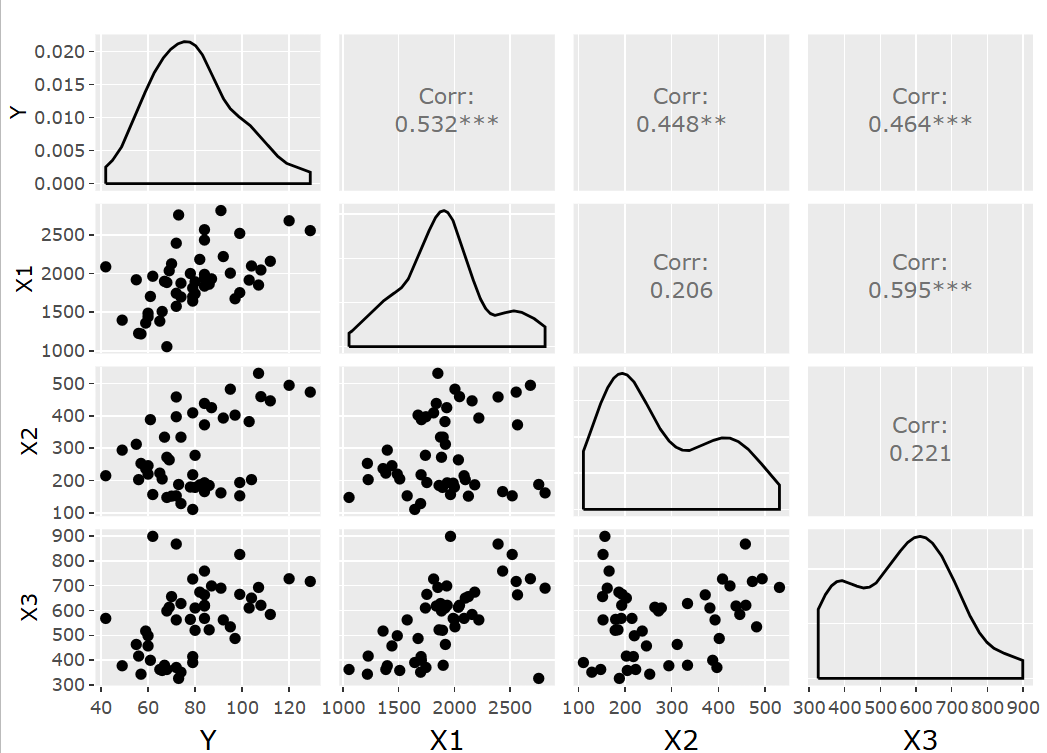
\includegraphics[width=0.5\textwidth]{plot_rel.png}
		\end{center}
		
		
		
		\vspace{.5cm}
		\item
		Please plot the relationship between \emph{Y} and \emph{Region}? On average, which region has the highest per capita expenditure on housing assistance?
		
		\begin{verbatim}
		expenditure$Region <- factor(expenditure$Region, 
									levels = c(1, 2, 3, 4),
									labels = c("North-East", "North Central", "South", "West"))
		
		ggplot(expenditure, aes(x=Region, y=Y, fill = Region)) + 
		geom_boxplot() +
		labs(y = "p/c expenditure on shelters/housing assistance", title = "p/c expenditure on shelters/housing assistance by Region")
		
		\end{verbatim}
		
		\textit{Answer: Based off the box plot results, the West has on average (via the median) the highest per capita expenditure on housing assistance.}
		
		\begin{center}
			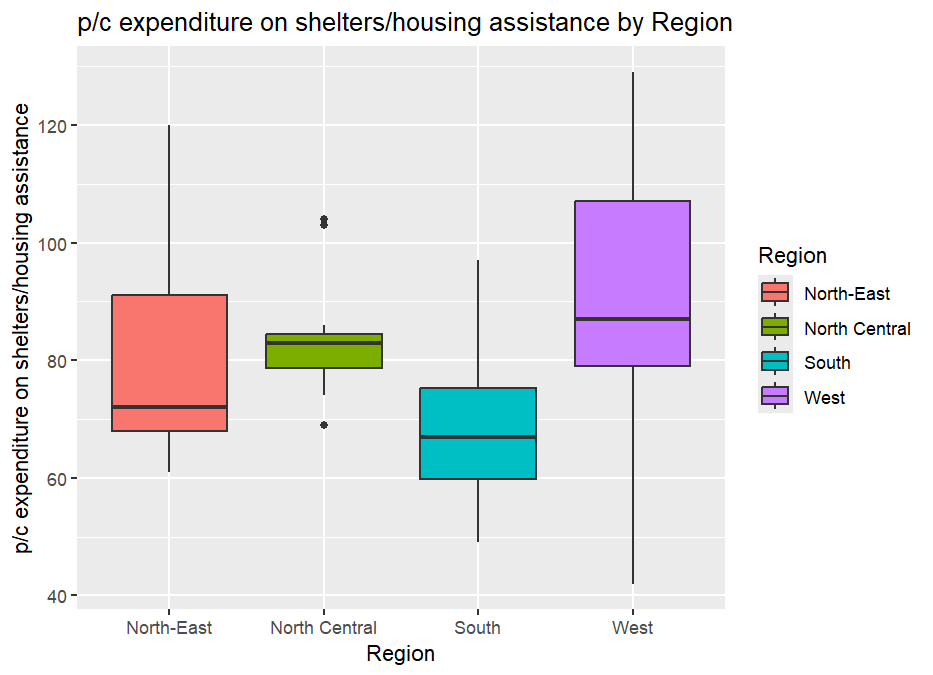
\includegraphics[width=0.5\textwidth]{region_box.png}
		\end{center}
		
		\vspace{.5cm}
		\item
		Please plot the relationship between \emph{Y} and \emph{X1}? Describe this graph and the relationship. Reproduce the above graph including one more variable \emph{Region} and display different regions with different types of symbols and colors.
		
		\textit{First the simple plot between Y and X1}
		
		\begin{verbatim}
			ggplot(expenditure, aes(x=X1, y=Y)) +
			geom_point() +
			geom_smooth( method=lm, se=FALSE) +
			labs(x = "p/c personal income in state", y = "p/c expenditure on housing assistance", title = "p/c expenditure on housing assistance by p/c personal income in state")
		\end{verbatim}
		
		\textit{Answer: The simple plot on the relationship between Y and X1 would demonstrate a relatively strong, positive and linear association between both variables. Outliers are minimal, and still fit with the strong directionality bar one value.}
		
		\begin{center}
			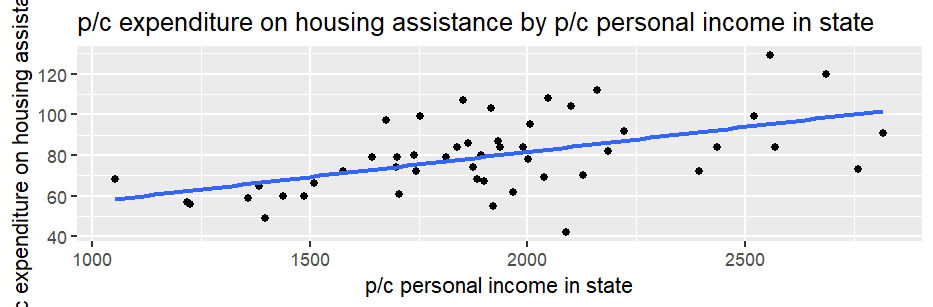
\includegraphics[width=0.5\textwidth]{Simple_plot.png}
		\end{center}
		
		\vspace{.5cm}
		\textit{Next the complex plot}
		\begin{verbatim}
			ggplot(expenditure, aes(x=X1, y=Y, shape= Region, colour = Region)) +
			geom_point() +
			labs(x = "p/c personal income in state", y = "p/c expenditure on shelters/housing", title = "p/c expenditure on housing assistance by p/c personal income in state") +
			geom_smooth( method=lm, se=FALSE)
		\end{verbatim}
		
		\textit{Answer: The more complex scatter plot, inclusive of region, demonstrates regional variation in association between both variables. The North-East in particular demonstrates quite a strong association, with observations quite close to the line. While the West - despite a clear positive linear association - contains the most outliers. The South appears to demonstrate the weakest association - though still positive. Notably its values skew heavily to the left.}
		
		\begin{center}
			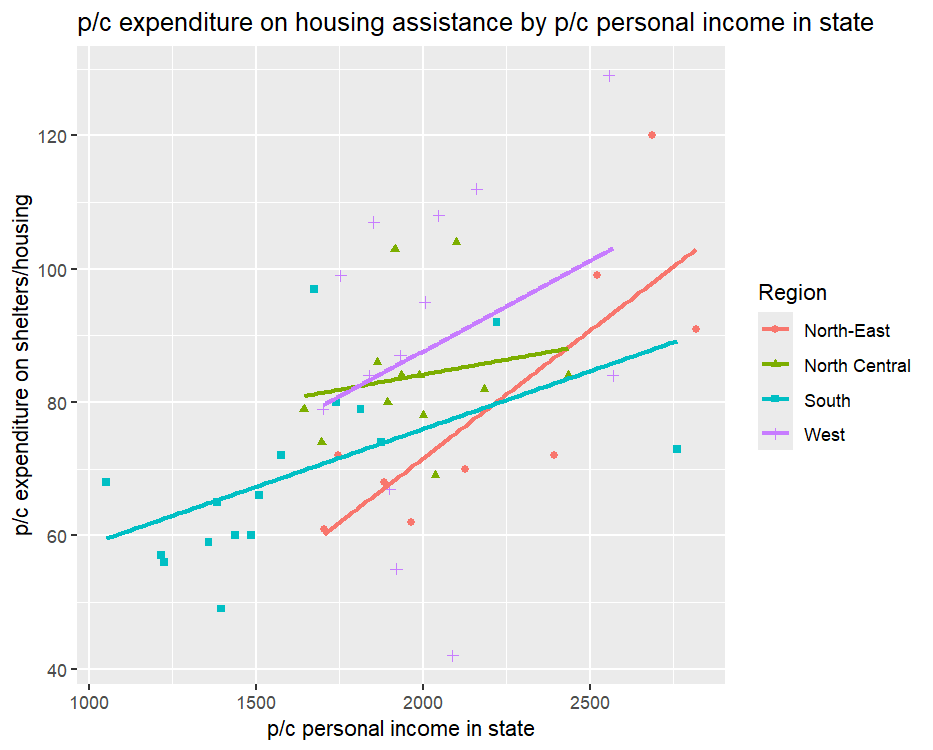
\includegraphics[width=0.5\textwidth]{Complex_plot.png}
		\end{center}
		
	\end{itemize}
	
	
\end{document}
